\documentclass[a4paper,11pt] {article}
% Default margins are too wide all the way around. I reset them here
\setlength{\topmargin}{.5in}
\setlength{\textheight}{9in}
\setlength{\oddsidemargin}{.125in}
\setlength{\textwidth}{6.25in}

\usepackage{color}
\usepackage[utf8]{inputenc}
\usepackage{graphicx}
\usepackage{float}
\usepackage{pdfpages}
\usepackage{amsthm}
\usepackage{amsmath,amsfonts,amssymb,amsthm}
\theoremstyle{definition}
\newtheorem{defn}{Definition}[section]
\newtheorem{conj}{Conjecture}[section]
\newtheorem{exmp}{Example}[section]

\definecolor{javared}{rgb}{0.6,0,0} % for strings
\definecolor{javagreen}{rgb}{0.25,0.5,0.35} % comments
\definecolor{javapurple}{rgb}{0.5,0,0.35} % keywords
\definecolor{javadocblue}{rgb}{0.25,0.35,0.75} % javadoc
%\usepackage[french]{babel}
\usepackage[T1]{fontenc}


\begin{document}
\title{\textbf{Usability and Skeuomorphism}}
\author{\textbf{Bodart Xavier} - \textbf{Chapeaux Thomas} - \textbf{Mayeur Bernard} \\
Université Libre de Bruxelles}

\maketitle
\begin{center}

\textbf{INFO-F501 Information technology in society} \\
Luc WILKIN
\end{center}
\begin{center}

~\\


\includegraphics[scale=0.15]{fig-report/ULBjea.jpg}
\end{center}

\begin{center}

\textit{“Most people make the mistake of thinking design is what it looks like. People think it’s this veneer – that the designers are handed this box and told, ‘Make it look good!’ That’s not what we think design is. It’s not just what it looks like and feels like. Design is how it works.” – Steve Jobs, New York Times 2003
\\}
\end{center}



\pagebreak
\tableofcontents
\pagebreak
\section{Introduction}

Most tools we use today, from wristwatches and squirt guns to smartphones and industrial softwares, rely on sophisticated technology hidden from the user. This require the user to be taught how to use the tool, which can be done with manuals and trial-and-error, but also by designing the tool in such a way that its usage is both obvious and simple.\\

While this has been done for centuries for physical objects using buttons, elaborate shapes, different materials, etc, the most recent computing devices tends to have a simplistic physical design (often reduced to a black surface with a touchscreen) and use software elements on the screen to interact with the user by touch, leaving the responsibility of design to the application creator.\\

According to recent market research (\cite{ABI-android}), the iPad from Apple is still the most sold tablet in the world. Its user base is so huge that several companies make their entire revenue by selling apps for it. In an App Store containing almost a million different apps (\cite{iOs61}), users trying to find an app for a particular use may find dozens of different iterations. Studying how to apply design principles in tablet application design may help to make an application easy to use and to understand, and thus standing out against competitors.\\

In this document, we concentrate on design trends in electronic tablet applications. In Sect.~\ref{sct:theory}, we present some of the basic design principles described in \cite{Norman02} which can be applied to the design of any object.\\

Then, in Sect.~\ref{sct:history}, we show how those principles can be recognized in the evolution of the design of computer systems, concluding with the current trends in electronic tablets, namely skeuomorphism and flat design.\\

Finally, in Sect.~\ref{sct:experiment}, we present experimentation results demonstrating how users react to those designs. One result is from our own experiment, in which we confronted various users to a skeuomorphic calculator application and to a flat one.\\

\section{Theoretical concepts and design principles}
When using an object, there could exist hundreds of way to interact with it. Design can be used to highlight the good usage of the object using two concept:
\begin{enumerate}
\item Perceived affordance in order to suggest the good alternatives
\item Constraints in order to limit the number of bad alternatives
\end{enumerate}

\label{sct:theory}

    \subsection{Perceived affordance}

Perceived affordance represents the quality of an object that suggest its utilization. This concept is very important in object-design due to the fact that it may represents the main source of information about the usage of the object. Indeed, people tends to not read the usage notice. In addition, this concept may reinforce the feeling of experience of a person for a given object.

\begin{figure}[h]
\centering
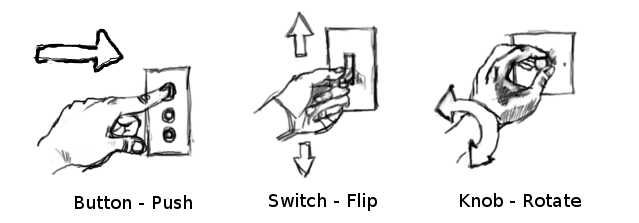
\includegraphics[scale=0.40]{fig-report/switches-only.png}
\caption{By their forms, buttons,switches or knobs often suggest their working.}
\end{figure}

Perceived affordance is not always the same as real affordance. Indeed, design can rarely explain the complete working of complex objects. The perceived affordance is only capable of showing primitive properties of its usage. Furthermore, a bad design may induce an usage more difficult than the correct design\cite{affordancesMads}.

\begin{figure}[h]
\centering
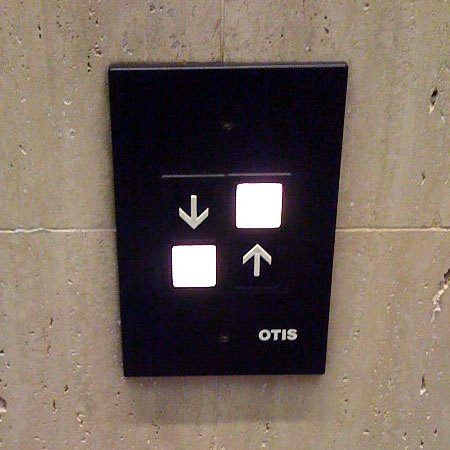
\includegraphics[scale=0.20]{fig-report/bad-switches.jpg}
\caption{What would you do in front of such a lift panel?}
\end{figure}

    \subsection{Natural mapping}
Natural mapping is the concept of organizing controllers in the same arrangement as the objects on which they have an influence to guarantee the expected result. This principle will often lead to an increase in perceived affordance.\\

A common example to illustrate this concept is the placement of the buttons that control the different stoves of your kitchen.It's obvious that the most left-top button will regulate the temperature of the most left-top stove.\\
 \begin{minipage}{\linewidth}
      \centering
      \begin{minipage}{0.45\linewidth}
          \begin{figure}[H]
          \centering
              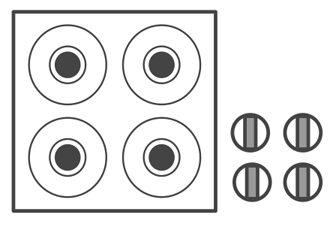
\includegraphics[scale=0.3]{fig-report/stove_natural.png}
              \caption{Scheme of a four stoves set with their corresponding knobs}
          \end{figure}
      \end{minipage}
      \hspace{0.05\linewidth}
      \begin{minipage}{0.45\linewidth}
          \begin{figure}[H]
                    \centering
              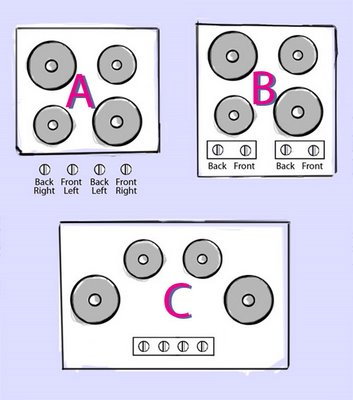
\includegraphics[scale=0.4]{fig-report/NormanBurners.jpg}
              \caption{These designs work only if you have the same assumption as the designer\cite{stoveMapping}}
          \end{figure}
      \end{minipage}
  \end{minipage}
  \bigskip


Unfortunately, this principle may sometimes induce extra design cost and may also depends on the point of view of the designer: even if it seems logical for certain arrangement such stoves or the control of the electronic windows of the car, one can still doubt about the mapping of light switches(\textit{"Does this switch controls  the lights of the front of the room because it is above the others ?"}).

    \subsection{Feedback}
\newtheorem{mydef}{Definition}
\begin{mydef}
\textit{\textbf{Feedback}}: sending back to the user information about what action has actually been done, what result has been accomplished.
\cite{Norman02}
\end{mydef}

In our case, feedback represents any action that could indicate to the user that its interaction with the item was taken into account. In certain cases, feedback can be done implicitly by the quality and the design of the object itself. For example, when a push button is  pressed, one can hear a clicking sound. On the other hand, feedback often requires, in our modern technologies, additional functions like vibrating or emitting sounds that corresponds to states of the device. Theses retro-actions have to provide enough information to the user in order to avoid his frustration about a mistaken usage.

\begin{figure}[h]
\centering
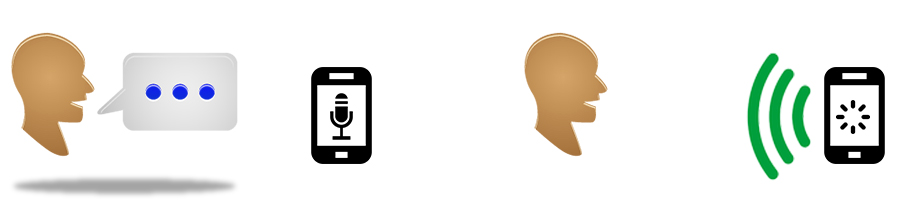
\includegraphics[scale=0.5]{fig-report/retro-action-speaking.jpg}
\caption{After the user gives a command, the device emits a sound to confirm that it is analysing the request}
\end{figure}

    \subsection{Additional design principles}

As presented in \cite{Norman02}, one can also add two principles to a good design:
\begin{itemize}
    \item \textbf{Provide a good conceptual model}: The idea is to provide a precise information model about the good usage of the object, or the way to maintain it. By following instructions, user should be guarantee to use the item correctly. The design of such scheme is really important and should be extremely clear. Indeed, if it's not, the user may be frustrated and not understand why it's not working.

    \item \textbf{Make things visible}: Certain of our modern items can be seen as real complex state machines due to the number of actions they can propose. The basic idea behind this principle is to provide a display which shows the current state and the available actions. A good example to this is the usage of a new VoIP telephone which allow a user to start a conference with several other people. Such telephone are often equipped with a large display which can show different contacts number, propose features to start conference or even to place a call on hold in order to answer to another call.
\end{itemize}

 \begin{minipage}{\linewidth}
      \centering
      \begin{minipage}{0.45\linewidth}
          \begin{figure}[H]
          \centering
              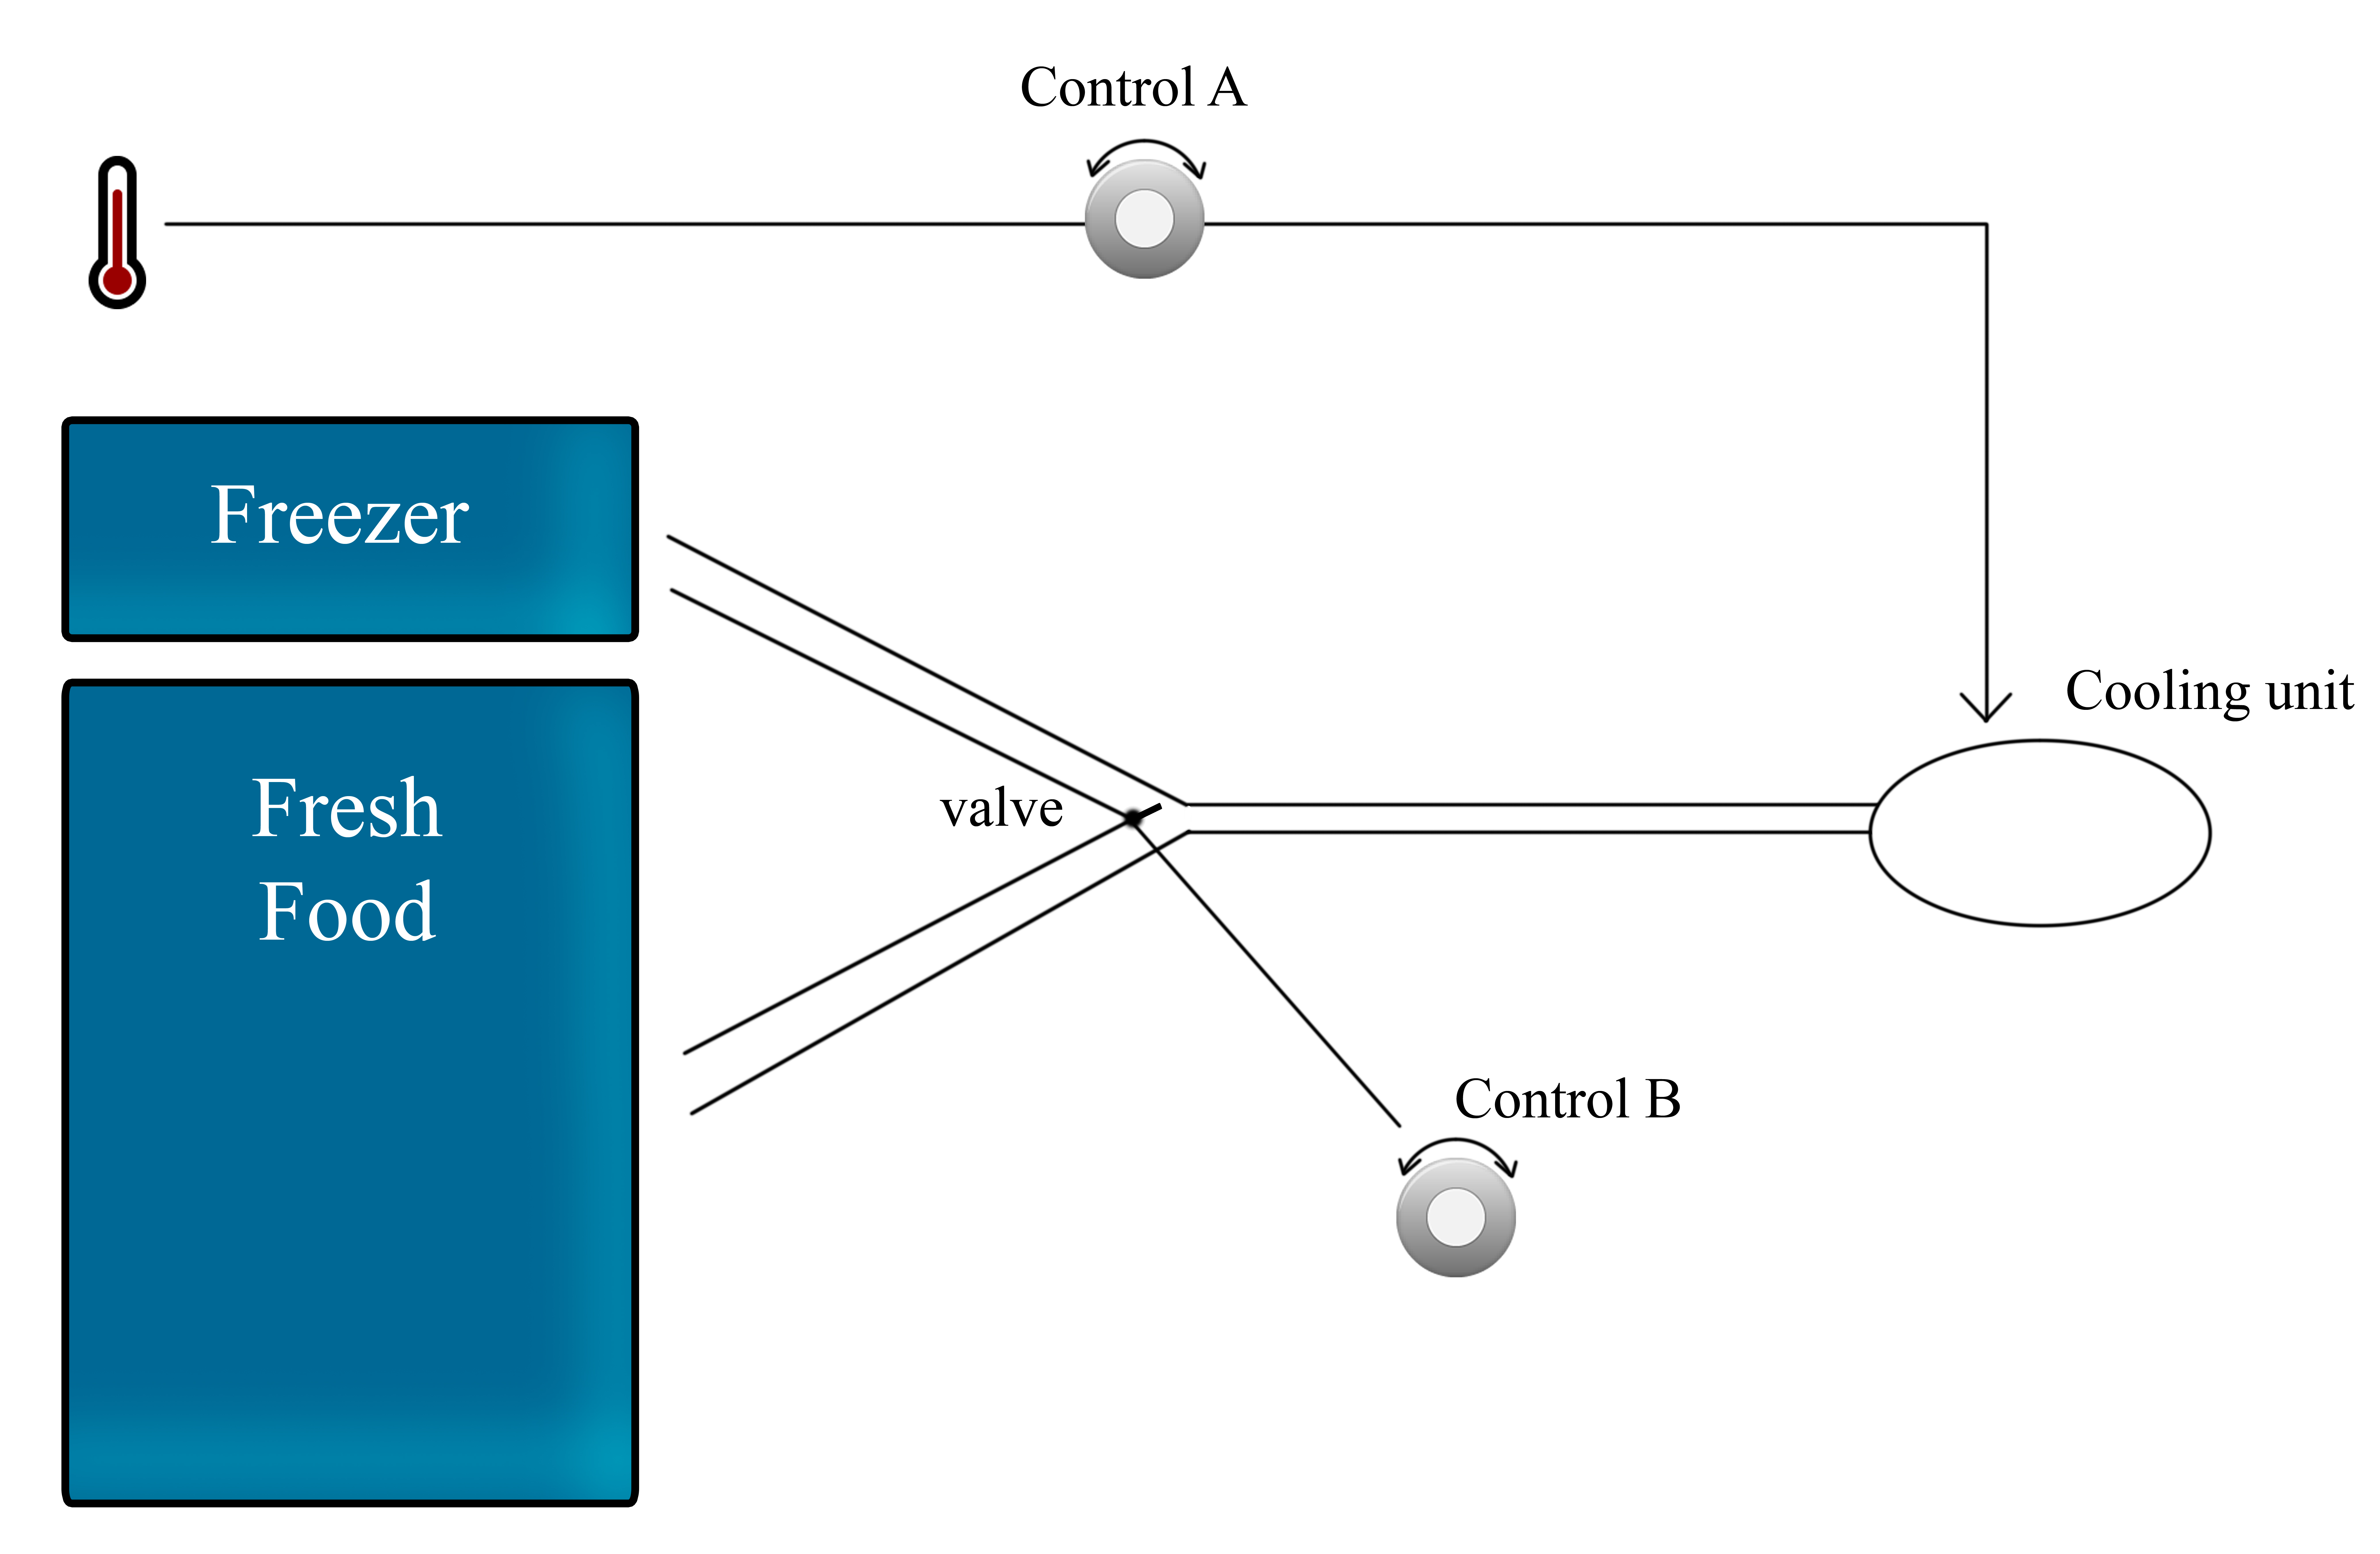
\includegraphics[scale=0.1]{fig-report/conceptual.jpg}
              \caption{The user can use control A to regulate temperature and control B to define the balance of cold air for the freezer and the fresh food. This scheme was inspired by a figure in  \cite{Norman02}}
          \end{figure}
      \end{minipage}
      \hspace{0.05\linewidth}
      \begin{minipage}{0.45\linewidth}
          \begin{figure}[H]
                    \centering
               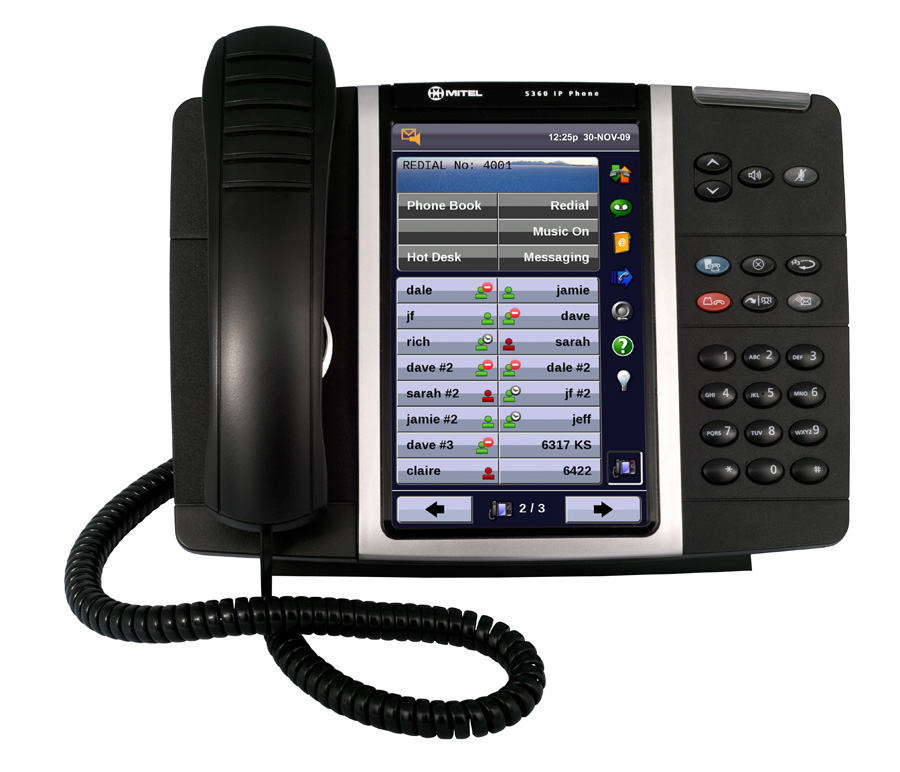
\includegraphics[scale=0.7]{fig-report/voip-phone.jpg}
              \caption{This VoIP phone has a big display to propose multiple commands}
          \end{figure}
      \end{minipage}
  \end{minipage}

    \subsection{Constraints}
    In addition to affordances, usage of objects is also induced by different types of constraints. These implicit rules may depend on the knowledge of the user but might increase perceived affordance. In the following subsections, each type of constraints will be explained and illustrated with an example.
        \subsubsection{Physical constraints}
        These constraints are the strongest ones because they reduce considerably the number of possible 	usages: Even without any attempt, the user will often be able to obviously discard  alternatives. They do not or poorly depend on the knowledge of the user.\\

        $\underline{Example:}$\\
        When a builder has just finished his work, he has to refill his toolbox which contains dedicated slots. Due to the design of the toolbox, it's completely impossible for him to put, for example, his hammer into the slot initially defined for a screwdriver.
        \begin{figure}[h]
        \centering
        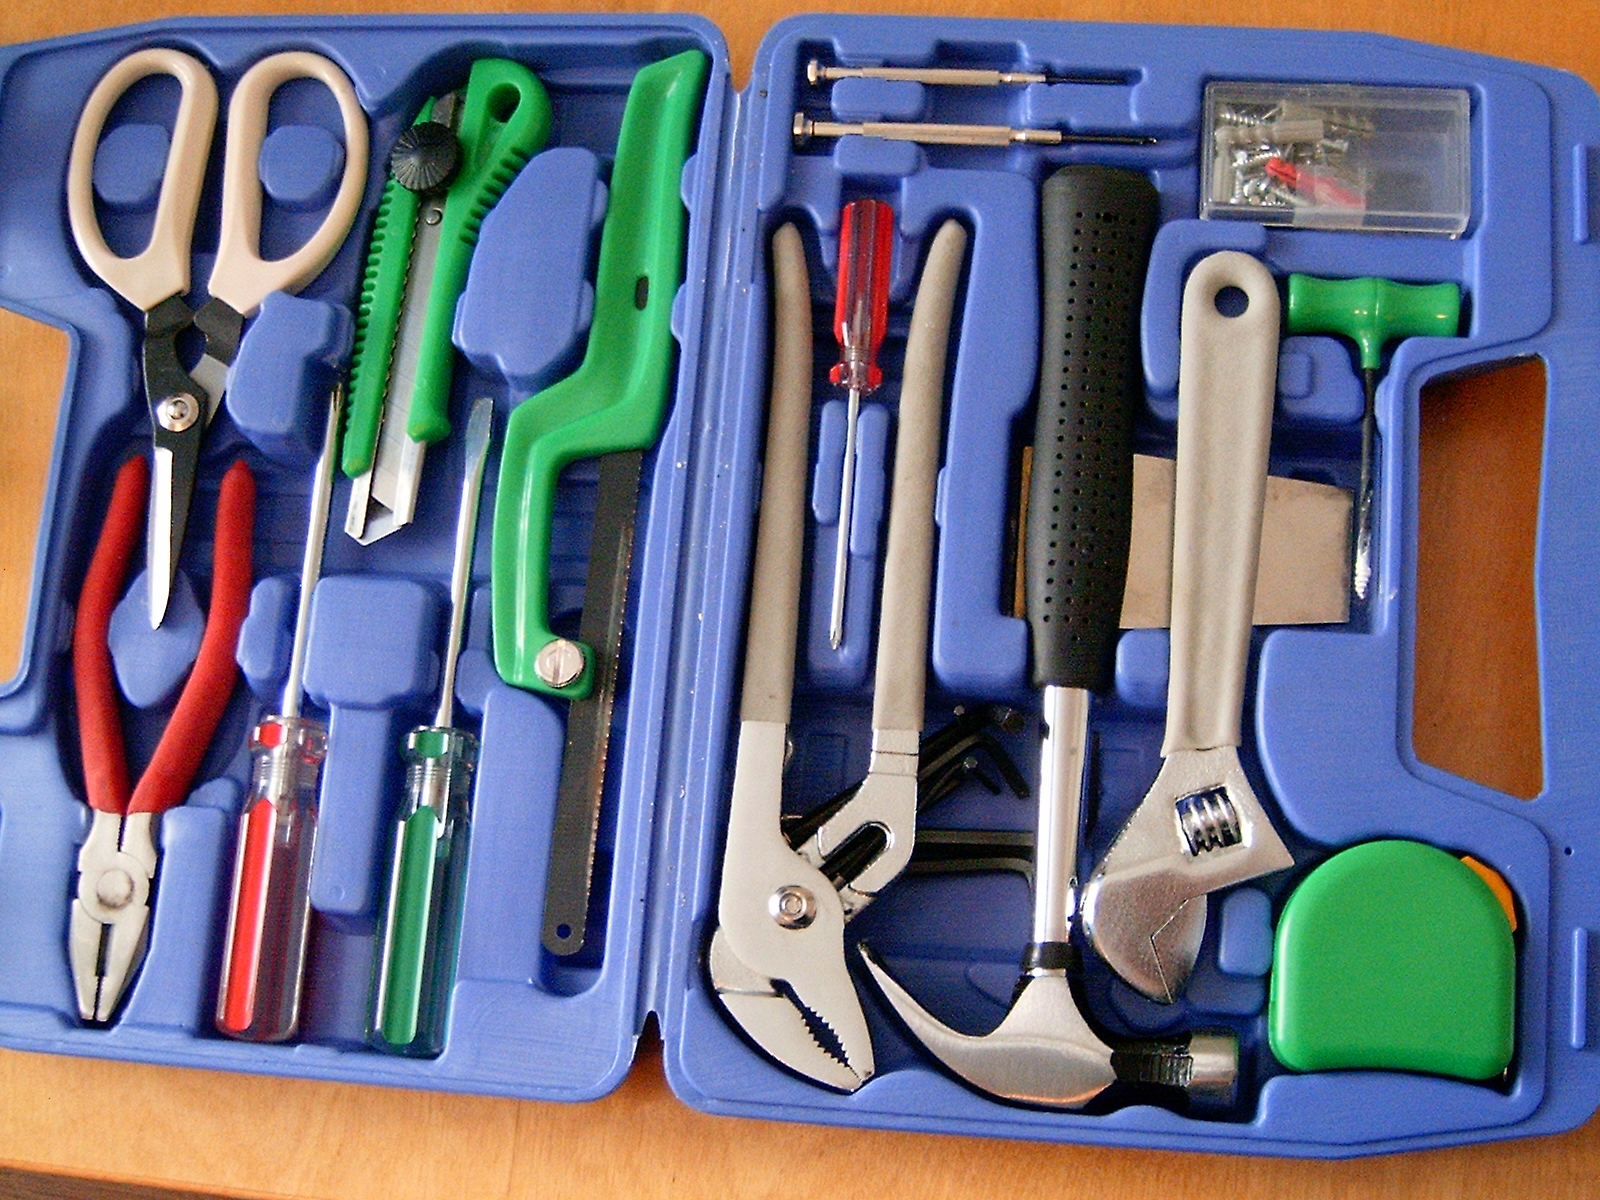
\includegraphics[scale=0.1]{fig-report/toolbox.jpg}
        \end{figure}

        \subsubsection{Semantic constraints}
       In opposition to the physical constraints, semantic constraints require a good knowledge of the situation in which the object should be used.\\

        $\underline{Example:}$\\
        It's difficult for a novice to do tie his shoes correctly the first time. After a while however, it appears simple and logical.
        \begin{figure}[h]
        \centering
        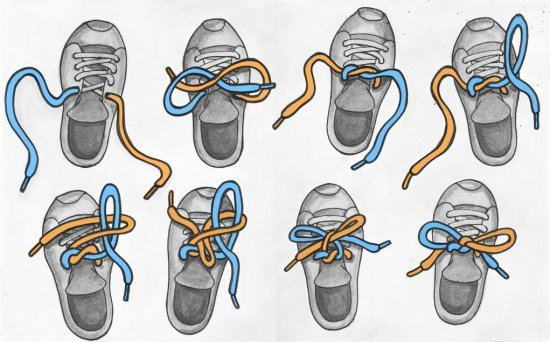
\includegraphics[scale=0.3]{fig-report/tie_your_shoes.jpg}
        \end{figure}

        \subsubsection{Cultural constraints}
        These constraints are the consequences of cultural conventions which have existed for several years. These constraints can be considered arbitrary because in most of the cases, several possible alternatives could be applicable. Indeed such constraints do not affect the semantic or the physical usage of the given object. Unfortunately, these constraints may change depending on the the geographical and temporal context. Furthermore, problems could arise when such constraints have to be decided for new items\\

        $\underline{Example:}$\\
        A basic example could be the disposition and the color of the traffic lights. In western countries, the green color represents the fact that you can go on and traffic lights are positioned in a vertical column . In Japan however, traffic lights may be composed of blue, orange and red lights, and could be displayed as a horizontal row.
        \begin{figure}[h]
        \centering
        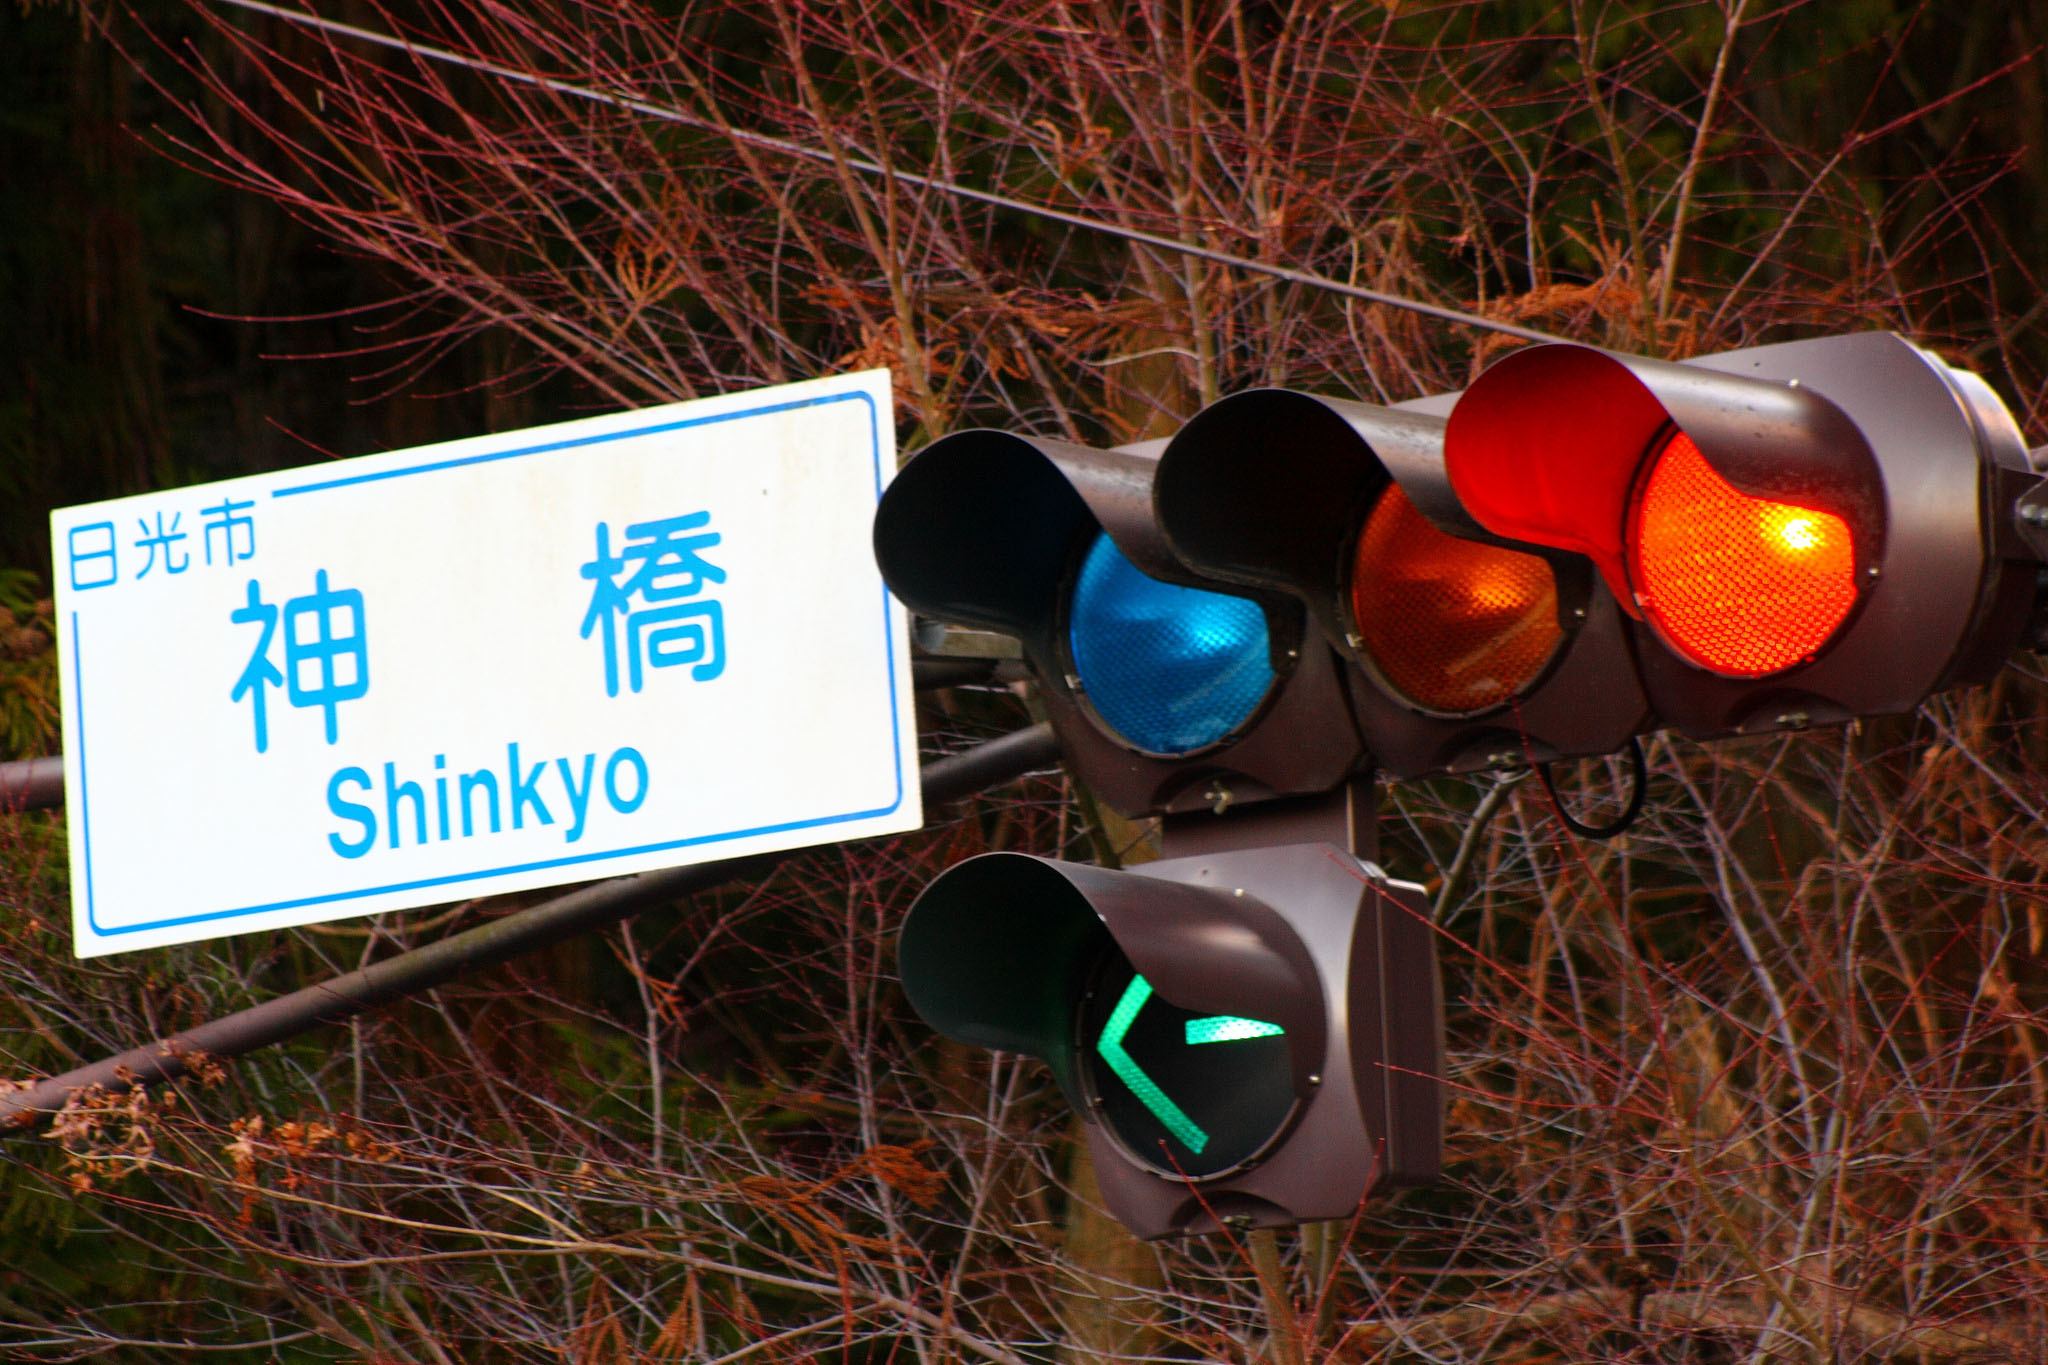
\includegraphics[scale=0.1]{fig-report/japan-traffic-light.jpg}
        \end{figure}

        \subsubsection{Logical constraints}
        These constraints call to the good-sense of the user. No physical or cultural knowledge is required here. The only thing that matters here is to confirm the first and logical assumption of user through design choices. Such constraints are often linked to natural mapping.\\

        $\underline{Example:}$\\
        The most trivial example could be the fact that a left switch will always activate the leftmost light.

\section{Evolution of computers interface}
\label{sct:history}

    \begin{figure}[h]
        \centering
        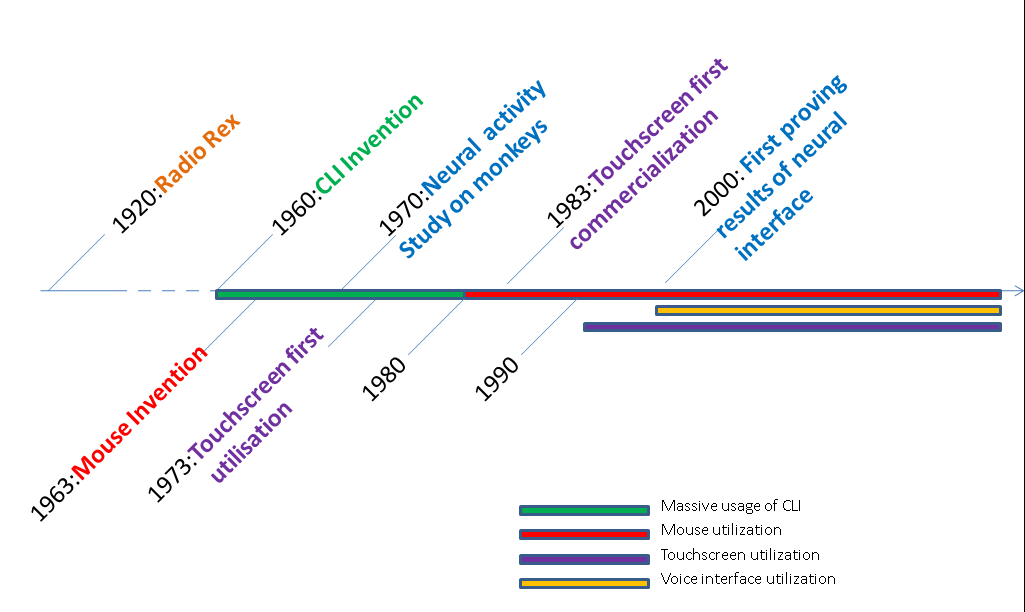
\includegraphics[width=0.75\textwidth]{fig-report/timeline-interface.png}
        \caption{Main events in the evolution of computer interfaces}
        \label{fig:timeline}
    \end{figure}

    As soon as computers became available to the public, the question of design came into play. While early designs were rough as computers were mainly aimed at professional use, the trend of personal computing brought a need for refined designs aimed at non-technical people. In this section, we present different types of computer interfaces for personal devices.

    \subsection{Command line interpreter (CLI)}

    \begin{figure}[h]
        \centering
        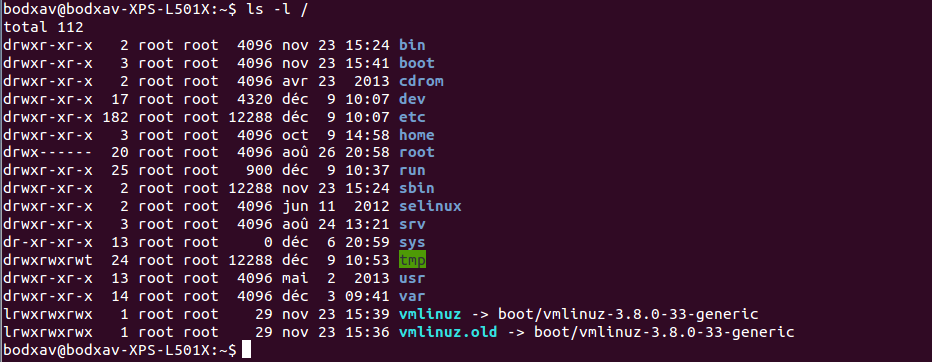
\includegraphics[width=0.75\textwidth]{fig-report/terminal.png}
        \caption{A typical CLI showing the content of a directory. Color is used for highlighting certain informations}
        \label{fig:cli}
    \end{figure}

    The first attempt at an usable design for computing devices was the command-line interface (abbreviated as CLI). The user can interact with the device using a keyboard by typing commands to launch programs, then the output of the program is displayed on the screen. While typing, the current command is displayed next to a cursor to provide feedback to the user. The buttons of the keyboard are labeled and follow a pattern standardized by countries, which is a case of natural mapping and cultural constraints.\\

    Command-line interfaces were introduced in the 1960s and remained a de-facto standard until the introduction of graphical interfaces. Later iterations were improved by features as auto-completion (which improved the perceived affordance of possible commands) and colors (which helped the user to build a conceptual model). Note that while CLI are not used as a main interface in personal computers anymore, advanced users still use it for some tasks for its efficiency.

    \subsection{Graphical interface and computer mouse}

    Invented in 1963 and made famous in 1968 during the ``Mother of All Demos''\cite{engelbart1968research}, the computer mouse, coupled with an OS using a graphical interface, allow the user to interact with the space of the screen. Graphical interfaces allowed designers to use powerful visual metaphors to construct an intuitive conceptual model (i.e. start button, trashbin, desktop, etc), as well as providing visual feedback to the user (movement of the mouse cursor, highlighting of selected items, animation when closing a program).\\

    Graphical interfaces and their intuitive conceptual model helped the broad adoption of personal computers.

    \subsection{Touch interface}
    \subsection{Voice interface}
    \subsection{Neural interface}
    \subsection{Current trends in touch interface}
        \subsubsection{Skeuomorphism}
        \subsubsection{Flat design}


\section{Experiments}
\label{sct:experiment}

    \subsection{Definition of the experiment}

    To compare skeuomorph and Flat design, we presented our subjects with two different calculator applications on iPad. One had a familiar skeuomorph design and the other had an original but intuitive design, based on Flat principles. After a quick demonstration of both apps, the subject was asked to answer simple questions using both applications. The quiz is available in appendix.\\

    % Figure showing the two apps...

    \subsection{Results analysis}
    
    During our experiments, people tends to choose the skeuomorph calculator for the first case, The travelling bill. Indeed, we suppose that due to simplicity of operations, people think the simpler calculator will be enough to solve every asked questions. A little problem arose, when we ask them to give us only the details for money spent on taxi fares due to the fact that the computation steps weren't labelled. In general, results provided by users were correct.\\
    
    In the second part of the experiment, we forced users to choose the other calculator(Most of the time, \textit{Soulver}). A first thing to notice, is the fact that most of users appeared to be lost due to uncommon interface. Indeed, numeric pad is not highlighted and Soulver proposes many other functions (such as percent computation, simple equation solving,\ldots). Instead of using dedicated functions, users tried to use their mathematical knowledge to solve given equations. As a consequence, results ( but also computation time) were not as good as in the first case. Once we showed them the additional functions in details, users appeared to be surprised but happy to see that the application integrates such features: Most of them explained us that they didn't see it because it's not emphasized and suggested that developed should use different types of buttons(color, shape, text color,\ldots). A good point of the flat calculator is the fact that it integrates a labelled history in which users can add textual information. This makes the "sub-resolution" problems easier.\\
    
    In general, users couldn't use the full potential of the flat calculator due to the lack of information. At first sight, and due to a limited designed, users appeared to be lost and limited their actions to the simplest one (addition, subtraction, division, multiplication) instead of exploiting the dedicated function to compute percentage or solve basic equation. Several users admitted that they wanted to use the flat calculator for everyday operations (shopping list, bills,\ldots) if they could follow a small training session.\\
    
    The last question of our poll was about the new design of IOS 7 proposed by \textit{Apple}.
    Users estimated that the new design( a flat design) is more beautiful and abstract without inducing a big loss in term of 	usability. The older users admitted that the a flat design required a necessary but fast adaptation:
  	(In french) \textit{Colette} - \textit{"Lors de la mise à jour, j'ai été surprise et un peu perdue parce que les toutes les icones avaient changer mais après 2-3 jours d'utilisation, je me suis adaptée. Si on devait revenir au précédent design, celà constituerait une perte de temps étant donné que je devrais m'y ré-adapaté."}
    
    

    \subsection{Comparison with previous studies}
    This is a subject where other studies are uncommon or mostly uncomplete. This make it difficult to compare, the three different studies that have been chosen and that will be exposed are: A blog about design that ask users about their preference, the windows 8 forum where a report over the preference between windows 7 and 8 is posted. Finally the last study is a japanese one, from the Department of Industrial Design National Cheng Kung University. This tries to analyse the different types of icons and class them between the abstact-concrete and detailled-terse factors.

    \subsubsection{Flat VS skeuomorphism\cite{flatVSskeuomorphisme}}
    This start with the survey, asking the users to give their preference between a set of icons from Google, IOS6, IOS7 and Windows phone. Here is the results :\\
    \begin{figure}[h]
    \centering
    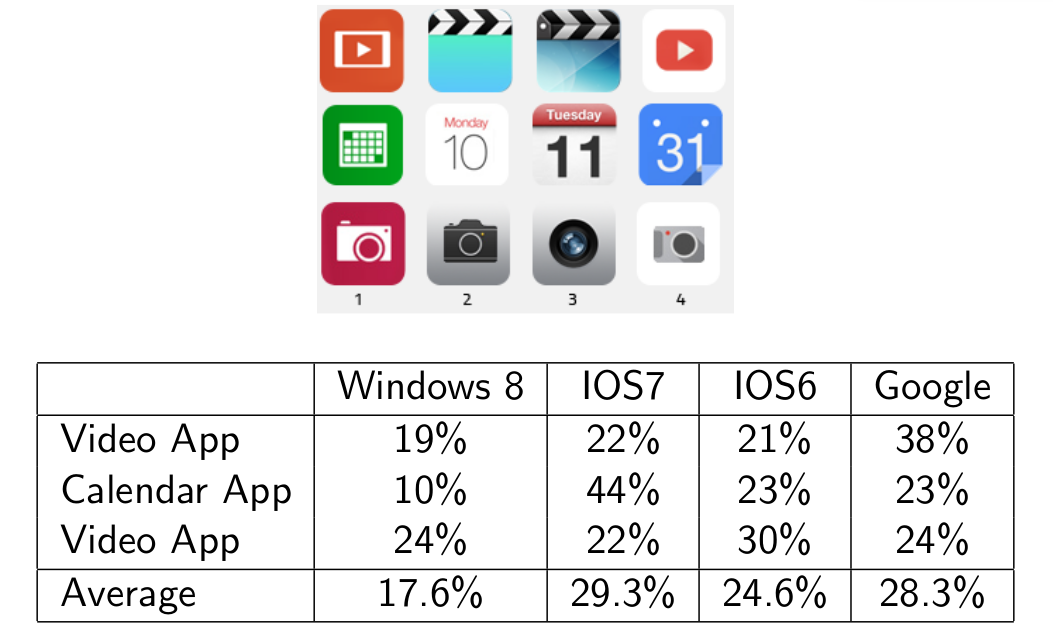
\includegraphics[scale=0.3]{fig-report/flatVSskeuomorphism.png}
    \end{figure}\\
As we can see, the results are not really significant, except if we consider that all except IOS6 are flat design, so that more than 70\% of the participant vote for flat design in each case. The main problem with this study is that there is no skeuomorph icons for google and windows phone. The majority of the icons beeing flat influance the results so that this is hard to belief. The second interresant thing is that windows 8 got a really low score for his calendar application. The three other possibilities looks similar and got an hier scores, leading to the conclusion that people really do not like this icon.

    \subsubsection{Windows 8 survey, half prefer windows 7\cite{windows8Survey}}
This survey is made by windows for windows users, and thus should be taken with care. After taking care of this, the informations revealed by the survey are quite interessant. The Metro UI (flat user interface) is classed in the 9th position of the most liked features with 22\% of the people liking it, while the fact to having two types of desktop, the Metro and the classical is disliked by 18\% of the people, putting it in the fifth place of the weaknesses to be improved.\\
We can ask ourself if the ones that voted for the Metro UI are not the same ones that voted for the double interface to be useless, because of the fact that the ones that are the most convincted of the flat interface should be the ones seeing a double interface to be the most usefull or ineffective.
\\
By summing all the votes, we can observe that on average, each voter has voted twice more for liked features than for weaknesses. Seeing that we could say that windows 8 is quite liked by the users of the forum. By remembering the fact that this survey is made on the windows 8 forum, that should be followed by the adepts of the windows operating system, we could rethink about it. Other surveys showered that in fact that two people still uses windows 7 for one using windows 8, a preference that could be caused by the price (35\% of the survey seeing this as one of the weaknesses) or lots of other factors that are not specially caused by the new UI. This makes it really hard to say which is prefered.
\\
The results stops by showing the corresponding graphs and graphs about the tablets. We should keep in mind that the results are from a windows 8 forum and that they are from september 2012, before we start to talk of IOS7 (september 2013). Globally, android leeds the maket whith one third of all mobile devices, one quarter of the cake was taken by IOS6 and windows one wuarter for the phones and one third for the tablets. This last information is interessant: while android and IOS globally get the same part of the market, windows seems to be prefered while on a bigger touchscreen device. This is caused by the fact that their new UI is thought to be used on flat, touchscreen computers and tablets. This is very representative and could lead to the conclusion that microsoft uses the flat design for other kind of devices, and thus should be used together instead of compare them.

    \subsubsection{A preliminary study on aesthetic of apps icon design\cite{jpAnalitics}}
This study is made by a Japanese university with the collaboration of two members of the Department of Industrial Design National Cheng Kung University in Taiwan. This try to analyse and determine the different aspects of the aesthetic in the icons, the links between themself and with the users and finaly investiguate the new issues to the skeuomorphism, meening the flat design. To get the results, they use evaluation grid results, quantification theory and regression to identify potential relationships between constituant of the icons. They also introduce the kansei interface concept that try to include the emotionnal principle in the UI.
\\
The kansei interface is a principle that gets the general principle of usability, but also add a positive emotion factor with what they call interactive motivation. This is used in the context of the app market, with lots of app doing the same things and where the need is to interest the user to look at your app, the icon beeing the representation of all the application behind it. It should create emotion to get the interest, motivation to look further, and usability to understand the purpose.
\\
The survey is make in three part, firstly designers that analysed the aestetic factor of the icons, secondly three of them decided the final aestetic structure of the icons. Finally 42 participant respond to a grid survey over they feeling of the icons. The figure \ref{jpfig5} in the appendix show the result of the second part.
\\
Third part begin with a questionnaire asking for the different type of icons to be attractive. The following results shows that more abstract it becomes, less attractive it is. We can also observe that concrete icons have more success than the abstract ones (flat).
\begin{figure}[H]
  \centering{
    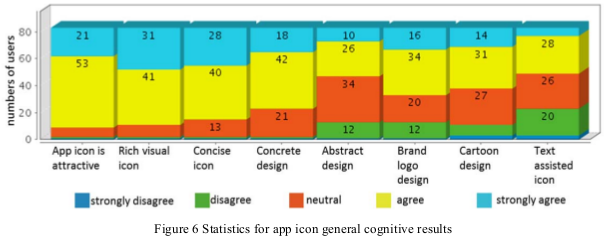
\includegraphics[scale=0.7]{fig-report/jpfig6.png}
  }
  \caption{Figure 6 of the study}\label{jpfig6}
\end{figure}
After this, a real questionnaire where given and the results were used to build a correlation between previously analysed factors and the fact that the icons where cute, vigorous,intuitive and fun. By example, to be vigorous, an icon should have a 3D effect, color, dynamic elements and novelty. The full table is present in the appendix, see figure \ref{jppage8}. This was made with the purpose of attempting to define the axis of the map as concrete-abstract and detailed-terse. See figure\ref{jpfig7}
\\
Based on the map, a second questionnaire were also done to compare the preference between concrete and abstract (or skeuomorph and flat design) icons. The results shows that most people prefer concrete style icons.
\begin{figure}[H]
  \centering{
    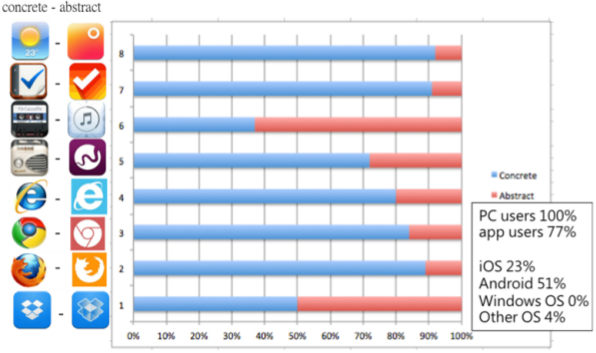
\includegraphics[scale=0.5]{fig-report/jppage10.png}
  }
  \caption{Results of the second questionnaire}\label{jppage10}
\end{figure}
    \subsubsection{Conclusion of the articles}
        The small quantity of source make it difficult to get a conclusion, but by referring to the two last ones, we could expect that our experiment would lead to a preference of the old, concrete style, where people knows how to make it work in comparison to a new flat design where will not find they mark
\section{Conclusion}

\newpage
\section{Appendix}
    \subsection{A preliminary study on aesthetic of apps icon design\cite{jpAnalitics}}
      \begin{figure}[H]
        \centering{
          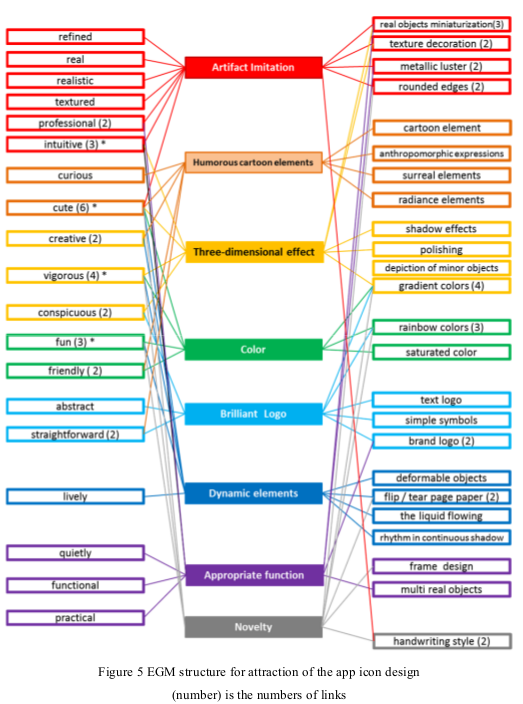
\includegraphics[scale=0.7]{fig-report/jpfig5.png}
        }
        \caption{Figure 5 of the study}\label{jpfig5}
      \end{figure}

      \begin{figure}[H]
        \centering{
          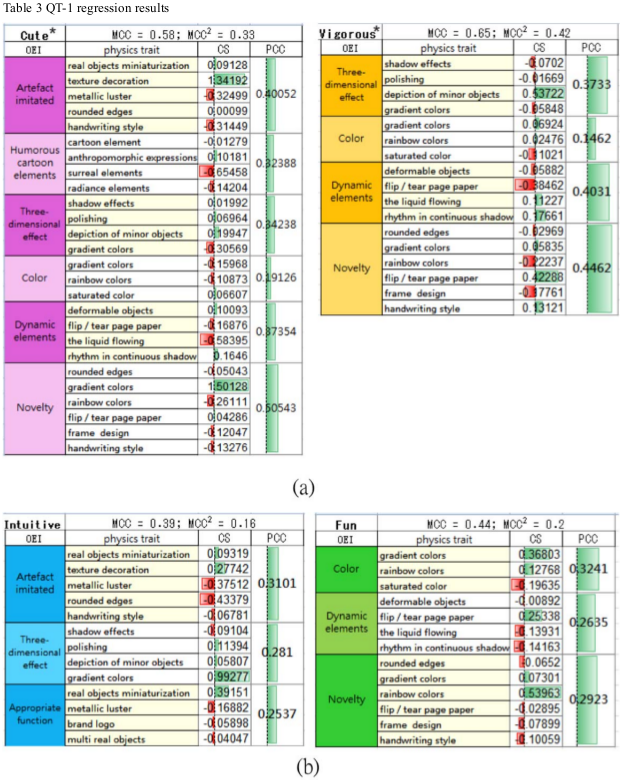
\includegraphics[scale=0.7]{fig-report/jppage8.png}
        }
        \caption{page 8 of the study}\label{jppage8}
      \end{figure}
      \begin{figure}[H]
        \centering{
          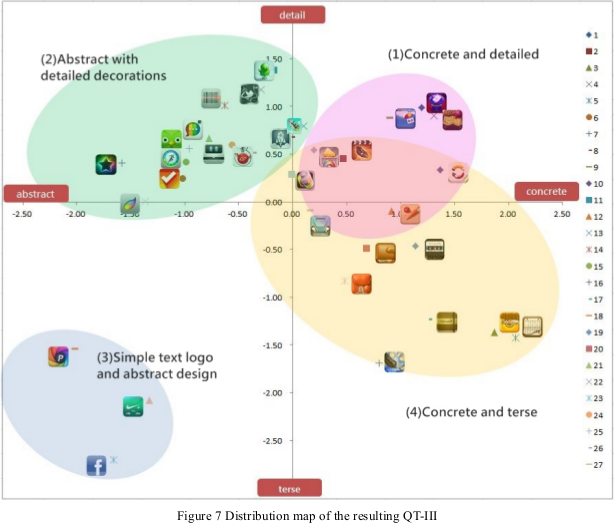
\includegraphics[scale=0.7]{fig-report/jpfig7.png}
        }
        \caption{Figure 7 of the study}\label{jpfig7}
      \end{figure}


\newpage
\bibliographystyle{plain}
\bibliography{bibUsability}
\end{document}
